\documentclass[12pt]{article}
\usepackage{amsmath,amsfonts,times}
\usepackage{graphicx,color,tikz,pgfplots}
\usepackage[paperwidth=15.8cm,paperheight=3.4cm,lmargin=0in,rmargin=0in,tmargin=0.in,bmargin=0.in]{geometry}
\usepackage{bm}
\usetikzlibrary{arrows,shadings,shapes.arrows,decorations.pathreplacing,calc, positioning}
\usepgfplotslibrary{fillbetween}


\newlength{\circleRadius}
\setlength{\circleRadius}{1.25pt}

\newlength{\cellWidth}
\setlength{\cellWidth}{3.2cm}

\newlength{\arrowLength}
\setlength{\arrowLength}{0.5cm}

\def\N{15}
\def\seed{6}

\begin{document}
\centering

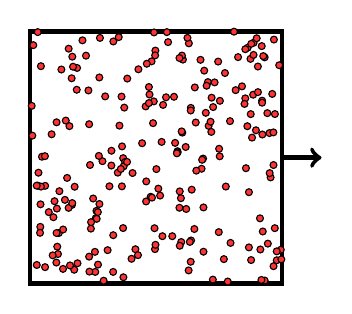
\begin{tikzpicture}[on grid]
  \draw[black,ultra thick] (0,0) rectangle (\cellWidth,\cellWidth);%marking borders
    
  % Lower left
  \pgfmathsetseed{\seed}
  \foreach \i in {1,...,\N}
  \fill[fill=red!80!white, draw=red!0!black] (0.2*rnd*\cellWidth, 0.25*rnd*\cellWidth) circle(\circleRadius);
  \foreach \i in {1,...,\N}
  \fill[fill=red!80!white, draw=red!0!black] (0.*\cellWidth + 0.2*rnd*\cellWidth, 0.25*\cellWidth + 0.15*rnd*\cellWidth) circle(\circleRadius);
  \foreach \i in {1,...,\N}
  \fill[fill=red!80!white, draw=red!0!black] (0.2*\cellWidth + 0.3*rnd*\cellWidth, 0.2*\cellWidth + 0.2*rnd*\cellWidth) circle(\circleRadius);
  \foreach \i in {1,...,\N}
  \fill[fill=red!80!white, draw=red!0!black] (0.2*\cellWidth + 0.3*rnd*\cellWidth, 0.2*rnd*\cellWidth) circle(\circleRadius);

  % Upper left
  \foreach \i in {1,...,\N}
  \fill[fill=red!80!white, draw=green!0!black] (0.3*rnd*\cellWidth, 0.4*\cellWidth + 0.35*rnd*\cellWidth) circle(\circleRadius);
  \foreach \i in {1,...,\N}
  \fill[fill=red!80!white, draw=green!0!black] (0.3*rnd*\cellWidth, 0.75*\cellWidth + 0.25*rnd*\cellWidth) circle(\circleRadius);
  \foreach \i in {1,...,\N}
  \fill[fill=red!80!white, draw=green!0!black] (0.3*\cellWidth + 0.2*rnd*\cellWidth, 0.4*\cellWidth + 0.3*rnd*\cellWidth) circle(\circleRadius);
  \foreach \i in {1,...,\N}
  \fill[fill=red!80!white, draw=green!0!black] (0.3*\cellWidth + 0.2*rnd*\cellWidth, 0.7*\cellWidth + 0.3*rnd*\cellWidth) circle(\circleRadius);

  % Lower right
  \foreach \i in {1,...,\N}
  \fill[fill=red!80!white, draw=red!0!black] (0.5*\cellWidth + 0.2*rnd*\cellWidth, 0.35*rnd*\cellWidth) circle(\circleRadius);
  \foreach \i in {1,...,\N}
  \fill[fill=red!80!white, draw=red!0!black] (0.5*\cellWidth + 0.2*rnd*\cellWidth, 0.35*\cellWidth + 0.25*rnd*\cellWidth) circle(\circleRadius);
  \foreach \i in {1,...,\N}
  \fill[fill=red!80!white, draw=red!0!black] (0.7*\cellWidth + 0.3*rnd*\cellWidth, 0.2*rnd*\cellWidth) circle(\circleRadius);
  \foreach \i in {1,...,\N}
  \fill[fill=red!80!white, draw=red!0!black] (0.7*\cellWidth + 0.3*rnd*\cellWidth, 0.2*\cellWidth + 0.4*rnd*\cellWidth) circle(\circleRadius);

  % Upper right
  \foreach \i in {1,...,\N}
  \fill[fill=red!80!white, draw=orange!0!black] (0.5*\cellWidth + 0.3*rnd*\cellWidth, 0.6*\cellWidth + 0.15*rnd*\cellWidth) circle(\circleRadius);
  \foreach \i in {1,...,\N}
  \fill[fill=red!80!white, draw=orange!0!black] (0.5*\cellWidth + 0.3*rnd*\cellWidth, 0.75*\cellWidth + 0.25*rnd*\cellWidth) circle(\circleRadius);
  \foreach \i in {1,...,\N}
  \fill[fill=red!80!white, draw=orange!0!black] (0.8*\cellWidth + 0.2*rnd*\cellWidth, 0.6*\cellWidth + 0.2*rnd*\cellWidth) circle(\circleRadius);
  \foreach \i in {1,...,\N}
  \fill[fill=red!80!white, draw=orange!0!black] (0.8*\cellWidth + 0.2*rnd*\cellWidth, 0.8*\cellWidth + 0.2*rnd*\cellWidth) circle(\circleRadius);

  % Arrow
  \draw[ultra thick, ->] (\cellWidth, 0.5\cellWidth) --++ (\arrowLength, 0);


\end{tikzpicture}
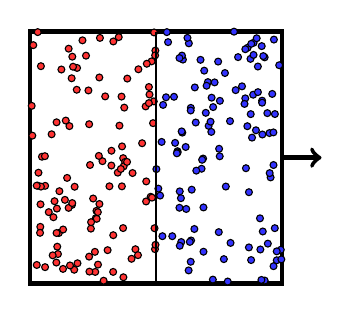
\begin{tikzpicture}[on grid]
  \draw[black,ultra thick] (0,0) rectangle (\cellWidth,\cellWidth);%marking borders
  
  % Lower left
  \pgfmathsetseed{\seed}
  \foreach \i in {1,...,\N}
  \fill[fill=red!80!white, draw=red!0!black] (0.2*rnd*\cellWidth, 0.25*rnd*\cellWidth) circle(\circleRadius);
  \foreach \i in {1,...,\N}
  \fill[fill=red!80!white, draw=red!0!black] (0.*\cellWidth + 0.2*rnd*\cellWidth, 0.25*\cellWidth + 0.15*rnd*\cellWidth) circle(\circleRadius);
  \foreach \i in {1,...,\N}
  \fill[fill=red!80!white, draw=red!0!black] (0.2*\cellWidth + 0.3*rnd*\cellWidth, 0.2*\cellWidth + 0.2*rnd*\cellWidth) circle(\circleRadius);
  \foreach \i in {1,...,\N}
  \fill[fill=red!80!white, draw=red!0!black] (0.2*\cellWidth + 0.3*rnd*\cellWidth, 0.2*rnd*\cellWidth) circle(\circleRadius);

  % Upper left
  \foreach \i in {1,...,\N}
  \fill[fill=red!80!white, draw=green!0!black] (0.3*rnd*\cellWidth, 0.4*\cellWidth + 0.35*rnd*\cellWidth) circle(\circleRadius);
  \foreach \i in {1,...,\N}
  \fill[fill=red!80!white, draw=green!0!black] (0.3*rnd*\cellWidth, 0.75*\cellWidth + 0.25*rnd*\cellWidth) circle(\circleRadius);
  \foreach \i in {1,...,\N}
  \fill[fill=red!80!white, draw=green!0!black] (0.3*\cellWidth + 0.2*rnd*\cellWidth, 0.4*\cellWidth + 0.3*rnd*\cellWidth) circle(\circleRadius);
  \foreach \i in {1,...,\N}
  \fill[fill=red!80!white, draw=green!0!black] (0.3*\cellWidth + 0.2*rnd*\cellWidth, 0.7*\cellWidth + 0.3*rnd*\cellWidth) circle(\circleRadius);

  % Lower right
  \foreach \i in {1,...,\N}
  \fill[fill=blue!80!white, draw=blue!0!black] (0.5*\cellWidth + 0.2*rnd*\cellWidth, 0.35*rnd*\cellWidth) circle(\circleRadius);
  \foreach \i in {1,...,\N}
  \fill[fill=blue!80!white, draw=blue!0!black] (0.5*\cellWidth + 0.2*rnd*\cellWidth, 0.35*\cellWidth + 0.25*rnd*\cellWidth) circle(\circleRadius);
  \foreach \i in {1,...,\N}
  \fill[fill=blue!80!white, draw=blue!0!black] (0.7*\cellWidth + 0.3*rnd*\cellWidth, 0.2*rnd*\cellWidth) circle(\circleRadius);
  \foreach \i in {1,...,\N}
  \fill[fill=blue!80!white, draw=blue!0!black] (0.7*\cellWidth + 0.3*rnd*\cellWidth, 0.2*\cellWidth + 0.4*rnd*\cellWidth) circle(\circleRadius);

  % Upper right
  \foreach \i in {1,...,\N}
  \fill[fill=blue!80!white, draw=orange!0!black] (0.5*\cellWidth + 0.3*rnd*\cellWidth, 0.6*\cellWidth + 0.15*rnd*\cellWidth) circle(\circleRadius);
  \foreach \i in {1,...,\N}
  \fill[fill=blue!80!white, draw=orange!0!black] (0.5*\cellWidth + 0.3*rnd*\cellWidth, 0.75*\cellWidth + 0.25*rnd*\cellWidth) circle(\circleRadius);
  \foreach \i in {1,...,\N}
  \fill[fill=blue!80!white, draw=orange!0!black] (0.8*\cellWidth + 0.2*rnd*\cellWidth, 0.6*\cellWidth + 0.2*rnd*\cellWidth) circle(\circleRadius);
  \foreach \i in {1,...,\N}
  \fill[fill=blue!80!white, draw=orange!0!black] (0.8*\cellWidth + 0.2*rnd*\cellWidth, 0.8*\cellWidth + 0.2*rnd*\cellWidth) circle(\circleRadius);


  % Medians
  \draw[black, thick, solid] (0.5*\cellWidth,0) -- ++ (0,1\cellWidth);
  %% \draw[black, thick, solid] (0,0.4\cellWidth) -- ++ (0.5\cellWidth, 0);
  %% \draw[black, thick, solid] (0.5\cellWidth,0.6\cellWidth) -- ++ (0.5\cellWidth, 0);

  % Arrow
  \draw[ultra thick, ->] (\cellWidth, 0.5\cellWidth) --++ (\arrowLength, 0);
\end{tikzpicture}
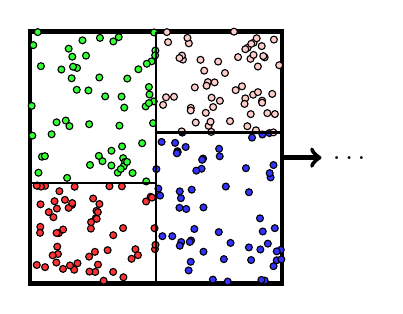
\begin{tikzpicture}[on grid]
  \draw[black,ultra thick] (0,0) rectangle (\cellWidth,\cellWidth);%marking borders

    % Lower left
  \pgfmathsetseed{\seed}
  \foreach \i in {1,...,\N}
  \fill[fill=red!80!white, draw=red!0!black] (0.2*rnd*\cellWidth, 0.25*rnd*\cellWidth) circle(\circleRadius);
  \foreach \i in {1,...,\N}
  \fill[fill=red!80!white, draw=red!0!black] (0.*\cellWidth + 0.2*rnd*\cellWidth, 0.25*\cellWidth + 0.15*rnd*\cellWidth) circle(\circleRadius);
  \foreach \i in {1,...,\N}
  \fill[fill=red!80!white, draw=red!0!black] (0.2*\cellWidth + 0.3*rnd*\cellWidth, 0.2*\cellWidth + 0.2*rnd*\cellWidth) circle(\circleRadius);
  \foreach \i in {1,...,\N}
  \fill[fill=red!80!white, draw=red!0!black] (0.2*\cellWidth + 0.3*rnd*\cellWidth, 0.2*rnd*\cellWidth) circle(\circleRadius);

  % Upper left
  \foreach \i in {1,...,\N}
  \fill[fill=green!80!white, draw=green!0!black] (0.3*rnd*\cellWidth, 0.4*\cellWidth + 0.35*rnd*\cellWidth) circle(\circleRadius);
  \foreach \i in {1,...,\N}
  \fill[fill=green!80!white, draw=green!0!black] (0.3*rnd*\cellWidth, 0.75*\cellWidth + 0.25*rnd*\cellWidth) circle(\circleRadius);
  \foreach \i in {1,...,\N}
  \fill[fill=green!80!white, draw=green!0!black] (0.3*\cellWidth + 0.2*rnd*\cellWidth, 0.4*\cellWidth + 0.3*rnd*\cellWidth) circle(\circleRadius);
  \foreach \i in {1,...,\N}
  \fill[fill=green!80!white, draw=green!0!black] (0.3*\cellWidth + 0.2*rnd*\cellWidth, 0.7*\cellWidth + 0.3*rnd*\cellWidth) circle(\circleRadius);

  % Lower right
  \foreach \i in {1,...,\N}
  \fill[fill=blue!80!white, draw=blue!0!black] (0.5*\cellWidth + 0.2*rnd*\cellWidth, 0.35*rnd*\cellWidth) circle(\circleRadius);
  \foreach \i in {1,...,\N}
  \fill[fill=blue!80!white, draw=blue!0!black] (0.5*\cellWidth + 0.2*rnd*\cellWidth, 0.35*\cellWidth + 0.25*rnd*\cellWidth) circle(\circleRadius);
  \foreach \i in {1,...,\N}
  \fill[fill=blue!80!white, draw=blue!0!black] (0.7*\cellWidth + 0.3*rnd*\cellWidth, 0.2*rnd*\cellWidth) circle(\circleRadius);
  \foreach \i in {1,...,\N}
  \fill[fill=blue!80!white, draw=blue!0!black] (0.7*\cellWidth + 0.3*rnd*\cellWidth, 0.2*\cellWidth + 0.4*rnd*\cellWidth) circle(\circleRadius);

  % Upper right
  \foreach \i in {1,...,\N}
  \fill[fill=pink!80!white, draw=orange!0!black] (0.5*\cellWidth + 0.3*rnd*\cellWidth, 0.6*\cellWidth + 0.15*rnd*\cellWidth) circle(\circleRadius);
  \foreach \i in {1,...,\N}
  \fill[fill=pink!80!white, draw=orange!0!black] (0.5*\cellWidth + 0.3*rnd*\cellWidth, 0.75*\cellWidth + 0.25*rnd*\cellWidth) circle(\circleRadius);
  \foreach \i in {1,...,\N}
  \fill[fill=pink!80!white, draw=orange!0!black] (0.8*\cellWidth + 0.2*rnd*\cellWidth, 0.6*\cellWidth + 0.2*rnd*\cellWidth) circle(\circleRadius);
  \foreach \i in {1,...,\N}
  \fill[fill=pink!80!white, draw=orange!0!black] (0.8*\cellWidth + 0.2*rnd*\cellWidth, 0.8*\cellWidth + 0.2*rnd*\cellWidth) circle(\circleRadius);


  % Medians
  \draw[black, thick, solid] (0.5*\cellWidth,0) -- ++ (0,1\cellWidth);
  \draw[black, thick, solid] (0,0.4\cellWidth) -- ++ (0.5\cellWidth, 0);
  \draw[black, thick, solid] (0.5\cellWidth,0.6\cellWidth) -- ++ (0.5\cellWidth, 0);


  %% \draw[black, thick, solid] (0.2\cellWidth,0) -- ++ (0, 0.4\cellWidth);
  %% \draw[black, thick, solid] (0.3\cellWidth,0.4\cellWidth) -- ++ (0, 0.6\cellWidth);

  %% \draw[black, thick, solid] (0.7\cellWidth,0) -- ++ (0, 0.6\cellWidth);
  %% \draw[black, thick, solid] (0.8\cellWidth,0.6\cellWidth) -- ++ (0, 0.4\cellWidth);

  %% % Lower left
  %% \draw[black, thick, solid] (0*\cellWidth,0.25\cellWidth) -- ++ (0.2\cellWidth, 0);
  %% \draw[black, thick, solid] (0.2*\cellWidth,0.2\cellWidth) -- ++ (0.3\cellWidth, 0);

  %% % Upper left
  %% \draw[black, thick, solid] (0*\cellWidth,0.75\cellWidth) -- ++ (0.3\cellWidth, 0);
  %% \draw[black, thick, solid] (0.3*\cellWidth,0.7\cellWidth) -- ++ (0.2\cellWidth, 0);

  %% % Lower right
  %% \draw[black, thick, solid] (0.5*\cellWidth,0.35\cellWidth) -- ++ (0.2\cellWidth, 0);
  %% \draw[black, thick, solid] (0.7*\cellWidth,0.2\cellWidth) -- ++ (0.3\cellWidth, 0);

  %% % Upper right
  %% \draw[black, thick, solid] (0.5*\cellWidth,0.75\cellWidth) -- ++ (0.3\cellWidth, 0);
  %% \draw[black, thick, solid] (0.8*\cellWidth,0.8\cellWidth) -- ++ (0.2\cellWidth, 0);
  
  % Arrow
  \draw[ultra thick, ->] (\cellWidth, 0.5\cellWidth) --++ (\arrowLength, 0) node[right] {$\ldots$};
\end{tikzpicture}
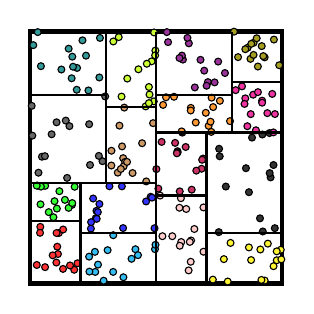
\begin{tikzpicture}[on grid, node distance=1em]
  \draw[black,ultra thick] (0,0) rectangle (\cellWidth,\cellWidth);%marking borders

  % Lower left
  \pgfmathsetseed{\seed}
  \foreach \i in {1,...,\N}
  \fill[fill=red!80!white, draw=red!0!black] (0.2*rnd*\cellWidth, 0.25*rnd*\cellWidth) circle(\circleRadius);
  \foreach \i in {1,...,\N}
  \fill[fill=green!80!white, draw=red!0!black] (0.*\cellWidth + 0.2*rnd*\cellWidth, 0.25*\cellWidth + 0.15*rnd*\cellWidth) circle(\circleRadius);
  \foreach \i in {1,...,\N}
  \fill[fill=blue!80!white, draw=red!0!black] (0.2*\cellWidth + 0.3*rnd*\cellWidth, 0.2*\cellWidth + 0.2*rnd*\cellWidth) circle(\circleRadius);
  \foreach \i in {1,...,\N}
  \fill[fill=cyan!80!white, draw=red!0!black] (0.2*\cellWidth + 0.3*rnd*\cellWidth, 0.2*rnd*\cellWidth) circle(\circleRadius);

  % Upper left
  \foreach \i in {1,...,\N}
  \fill[fill=darkgray!80!white, draw=green!0!black] (0.3*rnd*\cellWidth, 0.4*\cellWidth + 0.35*rnd*\cellWidth) circle(\circleRadius);
  \foreach \i in {1,...,\N}
  \fill[fill=teal!80!white, draw=green!0!black] (0.3*rnd*\cellWidth, 0.75*\cellWidth + 0.25*rnd*\cellWidth) circle(\circleRadius);
  \foreach \i in {1,...,\N}
  \fill[fill=brown!80!white, draw=green!0!black] (0.3*\cellWidth + 0.2*rnd*\cellWidth, 0.4*\cellWidth + 0.3*rnd*\cellWidth) circle(\circleRadius);
  \foreach \i in {1,...,\N}
  \fill[fill=lime!80!white, draw=green!0!black] (0.3*\cellWidth + 0.2*rnd*\cellWidth, 0.7*\cellWidth + 0.3*rnd*\cellWidth) circle(\circleRadius);

  % Lower right
  \foreach \i in {1,...,\N}
  \fill[fill=pink!80!white, draw=blue!0!black] (0.5*\cellWidth + 0.2*rnd*\cellWidth, 0.35*rnd*\cellWidth) circle(\circleRadius);
  \foreach \i in {1,...,\N}
  \fill[fill=purple!80!white, draw=blue!0!black] (0.5*\cellWidth + 0.2*rnd*\cellWidth, 0.35*\cellWidth + 0.25*rnd*\cellWidth) circle(\circleRadius);
  \foreach \i in {1,...,\N}
  \fill[fill=yellow!80!white, draw=blue!0!black] (0.7*\cellWidth + 0.3*rnd*\cellWidth, 0.2*rnd*\cellWidth) circle(\circleRadius);
  \foreach \i in {1,...,\N}
  \fill[fill=black!80!white, draw=blue!0!black] (0.7*\cellWidth + 0.3*rnd*\cellWidth, 0.2*\cellWidth + 0.4*rnd*\cellWidth) circle(\circleRadius);

  % Upper right
  \foreach \i in {1,...,\N}
  \fill[fill=orange!80!white, draw=orange!0!black] (0.5*\cellWidth + 0.3*rnd*\cellWidth, 0.6*\cellWidth + 0.15*rnd*\cellWidth) circle(\circleRadius);
  \foreach \i in {1,...,\N}
  \fill[fill=violet!80!white, draw=orange!0!black] (0.5*\cellWidth + 0.3*rnd*\cellWidth, 0.75*\cellWidth + 0.25*rnd*\cellWidth) circle(\circleRadius);
  \foreach \i in {1,...,\N}
  \fill[fill=magenta!80!white, draw=orange!0!black] (0.8*\cellWidth + 0.2*rnd*\cellWidth, 0.6*\cellWidth + 0.2*rnd*\cellWidth) circle(\circleRadius);
  \foreach \i in {1,...,\N}
  \fill[fill=olive!80!white, draw=orange!0!black] (0.8*\cellWidth + 0.2*rnd*\cellWidth, 0.8*\cellWidth + 0.2*rnd*\cellWidth) circle(\circleRadius);


  % Medians
  \draw[black, thick, solid] (0.5*\cellWidth,0) -- ++ (0,1\cellWidth);
  \draw[black, thick, solid] (0,0.4\cellWidth) -- ++ (0.5\cellWidth, 0);
  \draw[black, thick, solid] (0.5\cellWidth,0.6\cellWidth) -- ++ (0.5\cellWidth, 0);


  \draw[black, thick, solid] (0.2\cellWidth,0) -- ++ (0, 0.4\cellWidth);
  \draw[black, thick, solid] (0.3\cellWidth,0.4\cellWidth) -- ++ (0, 0.6\cellWidth);

  \draw[black, thick, solid] (0.7\cellWidth,0) -- ++ (0, 0.6\cellWidth);
  \draw[black, thick, solid] (0.8\cellWidth,0.6\cellWidth) -- ++ (0, 0.4\cellWidth);

  % Lower left
  \draw[black, thick, solid] (0*\cellWidth,0.25\cellWidth) -- ++ (0.2\cellWidth, 0);
  \draw[black, thick, solid] (0.2*\cellWidth,0.2\cellWidth) -- ++ (0.3\cellWidth, 0);

  % Upper left
  \draw[black, thick, solid] (0*\cellWidth,0.75\cellWidth) -- ++ (0.3\cellWidth, 0);
  \draw[black, thick, solid] (0.3*\cellWidth,0.7\cellWidth) -- ++ (0.2\cellWidth, 0);

  % Lower right
  \draw[black, thick, solid] (0.5*\cellWidth,0.35\cellWidth) -- ++ (0.2\cellWidth, 0);
  \draw[black, thick, solid] (0.7*\cellWidth,0.2\cellWidth) -- ++ (0.3\cellWidth, 0);

  % Upper right
  \draw[black, thick, solid] (0.5*\cellWidth,0.75\cellWidth) -- ++ (0.3\cellWidth, 0);
  \draw[black, thick, solid] (0.8*\cellWidth,0.8\cellWidth) -- ++ (0.2\cellWidth, 0);

  %% \draw[black, thick, solid] (0*\cellWidth,0.7\cellWidth) -- ++ (0.5\cellWidth, 0);
  %% \draw[black, thick, solid] (0.5*\cellWidth,0.8\cellWidth) -- ++ (0.5\cellWidth, 0);
\end{tikzpicture}

\end{document} 
